\section{Introduction}

SSU-ALIGN identifies and aligns small subunit ribosomal RNA
(SSU rRNA) genes in sequence datasets. It uses models of the primary
sequence and secondary structure conservation of SSU rRNA as inferred
by comparative sequence analysis and confirmed by crystal structure
determination from the \db{comparative rna website} (\db{crw}) 
(\url{http://www.rna.ccbb.utexas.edu/})
\cite{CannoneGutell02}.

\subsection{Overview}
The SSU-ALIGN package contains six different
programs: \prog{ssu-align}\footnote{SSU-ALIGN is the name of the
  software package as well as the name of one of the programs within
  the package. In this guide, when written in lowercase bold-faced
  type (\prog{ssu-align}) it refers to the executable program, and
  when written in all capital letters (SSU-ALIGN) it refers to
  the package.},
\prog{ssu-build}, \prog{ssu-draw}, 
\prog{ssu-mask}, \prog{ssu-merge}, and \prog{ssu-prep}. 

Suppose you have a dataset of SSU rRNA sequences from a PCR-based
environmental survey. You can use \prog{ssu-align} to create
structure-based multiple sequence alignments of the
SSU sequences using profile probabilistic models call covariance
models (CMs). \prog{ssu-align} will determine whether each sequence
is archaeal, bacterial or eukaryotic and output a multiple alignment
for each domain that was assigned at least one sequence. 
The \prog{ssu-mask} program can then be used to identify and remove
columns that are not reliably aligned. This step is important prior to using the
alignments as input to phylogenetic inference tools that rely heavily
on alignment accuracy.  
%Alignment columns are selected for removal
%based on automatically calculated ``confidence estimates'' for the
%aligned residues, which are the probabilities that each residue
%belongs in each column of the alignment given the CM. This is
%discussed in more detail in the section 3 of this guide.
The \prog{ssu-draw} program can be used to create secondary
structure diagrams of your alignments. Diagrams that display per-column
alignment statistics, such as information content and frequency of
insertions and deletions, as well as those that display individual
aligned sequences can be drawn.

The \prog{ssu-prep} and \prog{ssu-merge} programs allow users to
divide up large alignment jobs into sets of parallel
\prog{ssu-align} jobs on clusters or multi-core computers.

\prog{ssu-build} can be used to create different models than the
default archaeal, bacterial, and eukaryotic ones. For example, you
might want to build a model that represents a more specific
phylogenetic range, like the \emph{Firmicutes} bacterial phyla to
create maximally precise \emph{Firmicutes} SSU alignments. Or you can build
truncated versions of the default models that model only a
specific region of SSU, such as the V4 hypervariable region.

\subsection{ssu-align's search and alignment stages}

Given an input dataset of unaligned SSU sequences, \prog{ssu-align}
proceeds through two stages to generate alignments as depicted in
figure~\ref{fig:strategy}.  
%In stage 1, each of the sequences is aligned to each of
%the three models based on primary sequence conservation to obtain a
%score for each sequence to each model.  The model that gives the
%highest scoring alignment to each sequence is the \emph{best-matching
%  model} for that sequence.  In stage 2, each sequence is aligned to
%its best-matching model using both primary sequence and secondary
%structure conservation information. The end result is a separate
%multiple alignment for each model that was the best-matching model for
%at least one sequence in the input dataset.
In the first stage, each target sequence is scored with each of the
models based only on sequence conservation. This is done with a
profile HMM derived from each CM, which is significantly faster than
using the CM\@.  The model whose profile HMM gives the highest score to
each sequence is defined as the \emph{best-matching} model for that
sequence. If this highest score is not above a predefined threshold,
the sequence is discarded and not evaluated further. The boundaries of
the best-matching HMM alignment are used to truncate each target
sequence if the alignment does not span the entire target length.  In
stage 2, each surviving, and possibly truncated, sequence is aligned
to its best-matching model, this time using the CM which scores
both sequence and conserved structure. Up to $N$ alignments are
created, one for each model that was the best-match to at least one
target sequence.

\subsection{What distinguishes SSU-ALIGN from other SSU
  alignment tools}

%SSU-ALIGN is a freely available, open source software program
%for creating large-scale alignments of small subunit ribosomal RNA
%(SSU) using covariance models (CMs). The archaeal, bacterial,
%chloroplast, 
%and eukaryotic (nuclear) 
%and mitochondrial 
%SSU CMs in SSU-ALIGN are built from structural seed alignments derived from
%Robin Gutell's Comparative RNA Website (CRW) \cite{CannoneGutell02}.
%Though only a prototype which I hope to develop and extend in the
%future, 
%The following features distinguish SSU-ALIGN from other
%SSU alignment programs (reviewed in chapter 7 of \cite{Nawrocki09b}):

\begin{itemize}

\item \textbf{Structural alignments are calculated at roughly one
  second per sequence.}  

  CM alignment explicitly takes into account conserved sequence and
  well-nested structure. In the past, the slow speed of CM alignment
  has prevented their application to SSU alignment, but recent sequence-based
  acceleration heuristics \cite{Brown00,Nawrocki09b} have 
  made large-scale SSU CM alignment feasible.

\item \textbf{Alignment-specific masks for removing ambiguously aligned columns are
  automatically generated.}
  
  CMs are probabilistic models that allow calculation of the posterior
  probability that each sequence nucleotide belongs in each column of
  the output alignment given the model. Regions of low posterior
  probabilities are indicative of high alignment ambiguity and should
  be pruned away (masked out) prior to phylogenetic
  inference. \prog{ssu-mask} automatically detects and remove these
  columns for any alignment it generates. This is discussed in more
  detail in the section ~\ref{sec:background} of this guide.

\item \textbf{Accurate alignments can be computed using seed
  alignments of less than one hundred sequences.}

  CMs built from small seed alignments of dozens of sequences
  can achieve comparable accuracy to nearest-neighbor based alignment
  methods that use seed (reference) alignments of thousands or tens of
  thousands of sequences. This reduces the level of manual curation
  necessary for creating useful seeds, making it easier to extend
  SSU-ALIGN by adding new seeds and corresponding CMs that cover
  specific phylogenetic ranges. 

\end{itemize}


\subsection{What is included in this guide}

This user's guide is long. If you'd like to get started using the
software right away, take a look at section \ref{sec:install},
Installation and then section \ref{sec:tutorial}, Tutorial. You
can come back to the other sections later if you'd like.

Section~\ref{sec:install} describes how to install the
package. Section~\ref{sec:background} provides background information
on how SSU-ALIGN aligns SSU sequences, the distinction between
\emph{consensus} and \emph{insert} columns in its output alignments,
and how it identifies and removes columns from (masks) those
alignments.  The tutorial in section~\ref{sec:tutorial} walks through
examples of using the programs in SSU-ALIGN to create
alignments, mask alignments, build models of a specific region of SSU,
draw structure diagrams for alignments, and split up large alignment
jobs into smaller jobs to run in parallel on a cluster.
Section~\ref{sec:models} describes how the three default models were
derived from CRW. Section~\ref{sec:masks} details how the
default masks for the models were determined. 
Section~\ref{sec:stats} contains timing statistics and output file
sizes for aligning, masking and drawing various sized datasets.
Section~\ref{sec:output} describes the
format of output files generated by SSU-ALIGN programs.
Finally, the manual pages included at the end
of this guide explain the command-line options of the six programs.

\subsection{What is included in this package}

The six SSU-ALIGN programs: \prog{ssu-align}, \prog{ssu-build},
\prog{ssu-draw}, \prog{ssu-mask}, \prog{ssu-merge} and \prog{ssu-prep}
are PERL scripts.  The package includes the three default (archaea,
bacteria, and eukarya) SSU models and the \emph{seed} alignments they
were built from. These alignments were based on SSU structures and
alignments from the Comparative RNA Website (CRW)
\cite{CannoneGutell02}. A broader discussion of these models and
alignments and the specific procedure used to create them from the CRW
data is explained in section~\ref{sec:models}.

SSU-ALIGN bundles the INFERNAL software package, which is
written in C and is installed along with SSU-ALIGN by following
the directions in the Installation section of this
guide. INFERNAL itself includes Sean Eddy's HMMER package
and his sequence analysis library EASEL. All of the programs in
INFERNAL as well as small-scale EASEL applications for sequence
file manipulations are installed with SSU-ALIGN. Importantly, the
versions of the INFERNAL and EASEL programs get renamed and given a
\prog{ssu-} prefix to avoid namespace clashing with programs of the
same names if you have INFERNAL installed on your system. For example,
\prog{cmsearch} and \prog{esl-seqstat} as installed with SSU-ALIGN are
actually called \prog{ssu-cmsearch} and \prog{ssu-esl-seqstat}.

\subsection{What this package depends on}
SSU-ALIGN was developed and tested on Mac OS/X and Linux
(Redhat), but it should work on most UNIX platforms. It requires a C
compiler and PERL (Practical Extraction and Report
Language, Larry Wall) interpreter package version 5.0 or later.  No
other programs or libraries are required. If the program \prog{ps2pdf}
is installed on your system and in your PATH, \prog{ssu-draw} and
\prog{ssu-mask} will use it to convert postscript diagrams to PDF, but
it is not required.

\subsection{What this package does not do}

SSU-ALIGN only creates alignments, masks them, and draws SSU
secondary structure diagrams; it does not infer trees from the
alignments it creates, nor does it classify sequences beyond reporting
which model in the input CM file they score highest to.

\begin{comment}
\subsection{Other useful references}

The INFERNAL user's guide \cite{infernalguide} included in
this package supplements this user's guide. My Ph.D. thesis 
(\url{http://eddylab.org/publications.html})
introduces and describes my work on CM methods. It includes three chapters (7-9) dedicated to
SSU rRNA alignment; chapter 9 is included in this guide as
section~\ref{section:chap9}, but the other chapters may include some
relevant background information as well. 
Other useful references on CMs include
\cite{Eddy94,Durbin98,Eddy02b,NawrockiEddy07,Nawrocki09,KolbeEddy09}. In
addition, the \database{rfam} database 
(\url{http://rfam.sanger.ac.uk/})
uses INFERNAL to search for and align
structural RNAs using more than 1000 different CMs, so its
publications may be of interest as well
\cite{Griffiths-Jones03,Griffiths-Jones05,Gardner09}.
\end{comment}

\subsection{How to cite SSU-ALIGN}

SSU-ALIGN does not yet have an associated publication,
so please cite the INFERNAL software publication
(\cite{Nawrocki09}) if you find the package useful for work that
you publish. Additionally, because SSU-ALIGN's seed alignments were
derived from the \db{comparative rna website} we ask that you cite
that database as well: \cite{CannoneGutell02}. 
%Finally, if you'd like to, you
%can also cite my Ph.D. thesis \cite{Nawrocki09b} because it is
%currently the most relevant and comprehensive reference for the
%program.

\subsection{Future development}

We consider version 0.1 of SSU-ALIGN to be a prototype. 
Compute time for alignment is roughly one second per full length SSU
sequence. We hope to speed up the program and add additional SSU
models in future releases. Bug reports and feature requests are
appreciated.



\begin{figure}
  \begin{center}
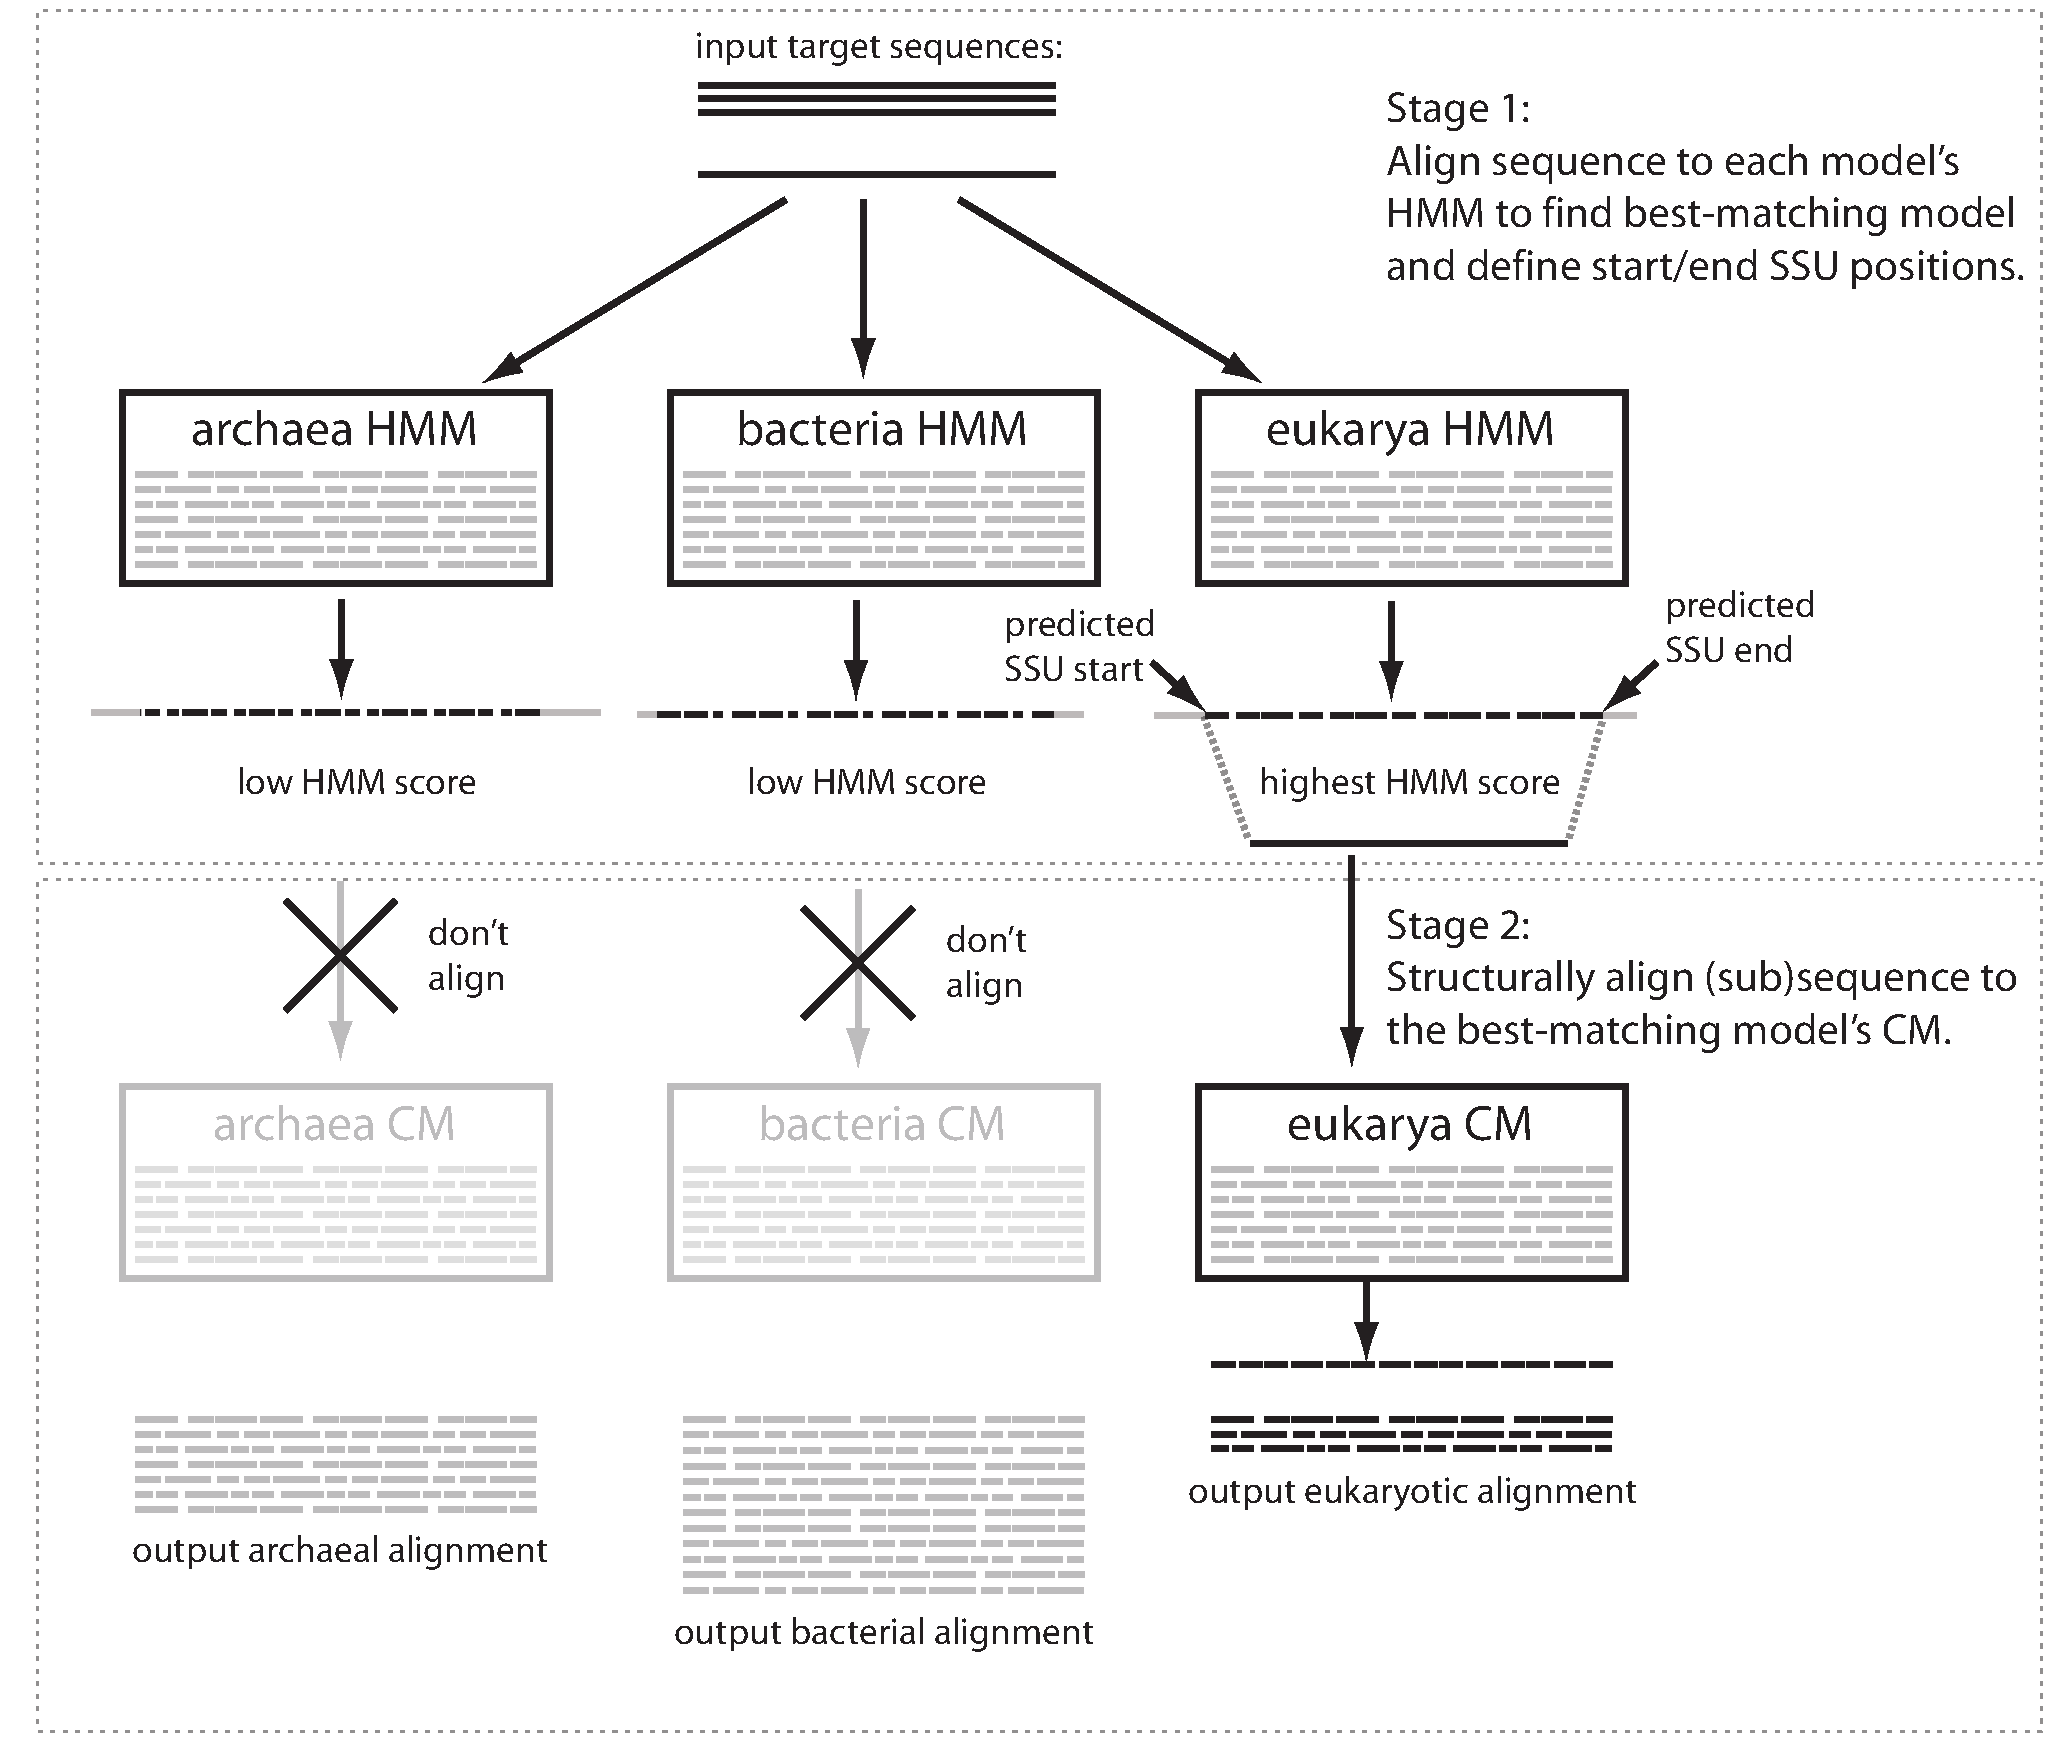
\includegraphics[width=6.5in]{Figures/ssualign-schematic}
  \end{center}
\caption{\textbf{Schematic of the \prog{ssu-align} alignment
    pipeline.} Unaligned target sequences are input to the
  program. In stage 1, each sequence is independently aligned
  using only primary sequence scoring to each of $N$ HMMs (by
  default, $N$ is 3), one built from each model in the input
  CM file. The model whose HMM alignment has the maximum bit
  score is the ``best-matching'' model for that sequence, in
  this example ``eukarya'' is the best-matching model. In
  stage 2, the unaligned (sub)sequence from the best-matching
  model's HMM alignment (potentially with some sequence
  trimmed off the ends) is aligned to the best-matching
  model's CM which scores both sequence and conserved
  secondary structure. The CM aligned target sequence is added
  to that model's output alignment. After all target sequences
  are processed, the program has output up to $N$ new
  structural alignments, one for each model that was the
  best-matching model for at least 1 target sequence.}
\label{fig:strategy}
\end{figure}
